\section{The reduced-envelope 25-move construction}\label{app:route25}

This construction records only those cells whose freedom from Breaker
is not already implied by Maker's required holdings.  It gives a second
finite strategy, with a different placement convention and a different
opening cover.  We first justify this representation and its exact
relationship to Section~\ref{sec:calculus}, then reconstruct the
certificate and explain its elementary and nonlocal attacks.

Throughout this appendix, a numbered \emph{$25$-card} belongs to the
family
\[
 \mathsf C^{25}_i=(P_i,E_i,h_i),\qquad 0\leq i\leq2015.
\]
The symbols $P_i,E_i,h_i$ in this appendix refer only to that family.
Its card numbers, placement codes, and local coordinates are independent
of the $21$- and $35$-move constructions.  In particular, their cards
with the same number need not have the same sets or meaning.

\subsection{Reduced requirements and their normalization}
\label{r25:semantics}

Let $P,E\subset\Z^2$ be finite and let $h\geq1$ be an integer.  A
\emph{valid reduced card} $(P,E,h)$ means the following: at every Maker turn with
finite disjoint ownership sets $M,B$, if
\begin{equation}\label{r25:condition}
 P\subseteq M,\qquad B\cap E=\varnothing,
\end{equation}
Maker has already won or can win within $h$ further actual Maker
claims.  We do not impose $P\subseteq E$, nor do we require $P$ and
$E$ to be disjoint.  Additional Maker cells and arbitrary Breaker
cells outside $E$ are allowed.  A signed permutation and translation
applied to both sets preserves validity and height, by the same
transport argument as for full cards.

The normalization
\begin{equation}\label{r25:normalization}
 (P,E,h)\longmapsto (A,T,h)=(P,P\cup E,h)
\end{equation}
preserves exactly the admissible positions.  Indeed, $P\subseteq M$
and $M\cap B=\varnothing$ already imply $B\cap P=\varnothing$;
under that assumption,
\[
 B\cap E=\varnothing
 \quad\Longleftrightarrow\quad
 B\cap(P\cup E)=\varnothing.
\]
Conversely, a full card $(A,T,h)$ with $A\subseteq T$ has the reduced
representative $(A,T\setminus A,h)$.  Normalizing this representative
returns $(A,T,h)$ exactly.  Normalizing an arbitrary $(P,E,h)$ and then
reducing replaces $E$ by $E\setminus P$; this changes no hypothesis
on a legal position.  Thus disjoint reduced sets are convenient
representatives, not an extra assumption in the semantics.

\begin{proposition}[Reduced composition]\label{r25:composition}
Let $(P_j,E_j,h_j)$, $1\leq j\leq m$, be valid reduced cards already
placed in one coordinate plane, where $1\leq m<\infty$.  Given an
attack cell $x$, put
\begin{equation}\label{r25:reduced-rule}
 \begin{aligned}
 U&=\bigcup_jP_j,& V&=\bigcup_jE_j,& I&=\bigcap_jE_j,\\
 H&=U\cup I,& P&=H\setminus\{x\},&
 E&=(V\setminus H)\cup\{x\},\qquad
 h=1+\max_jh_j.
 \end{aligned}
\end{equation}
Then $(P,E,h)$ is valid.  Its normalization is exactly the full card
obtained by Lemma~\ref{thm:composition} from the normalized children
$(P_j,P_j\cup E_j,h_j)$ at $x$; in particular, normalization changes
neither the required set nor the height.
\end{proposition}

\begin{proof}
We give the direct game argument, including the move that is needed
when the attack cell is already owned.  Suppose~\eqref{r25:condition}
holds for the parent and no target is complete.  Because $x\in E$,
Breaker does not own $x$.  If it is free, claim it.  Otherwise Maker
already owns it and claims any free cell instead; finite ownership on
$\Z^2$ guarantees that one exists.  This replacement consumes one
actual Maker claim, with its ensuing Breaker reply if play continues.
In either case the new Maker set $M'$ contains $H$, since it contains
$P$ and $x$.

Every older Breaker cell avoids every child envelope $E_j$.  To see
this without assuming $P_j\subseteq E_j$, note that the cells of $E_j$
outside $H$ lie in $E$, while its cells inside $H$ now belong to
Maker.  If the move has not won, the next legal Breaker cell $b$ is
outside $M'$, hence outside $I\subseteq H$.  Since the child list is
nonempty, some $E_j$ omits $b$.  At the next Maker turn this child
satisfies
\[
 P_j\subseteq U\subseteq M',\qquad
 (B\cup\{b\})\cap E_j=\varnothing.
\]
It wins in at most $h_j$ additional Maker claims.  The total is at most
$1+h_j\leq h$.  This also covers replies anywhere outside the finite
sets displayed in the construction.

For the asserted exact agreement, the pointwise identity is
\begin{equation}\label{r25:intersection-identity}
 U\cup\bigcap_j(P_j\cup E_j)
   =U\cup\bigcap_j E_j=H.
\end{equation}
For a point outside $U$, membership in $P_j\cup E_j$ is equivalent
to membership in $E_j$ for every $j$; points inside $U$ belong to both
sides.  This proves the identity without any containment or
disjointness assumption on the child sets.  Consequently the full
composition's required set is $H\setminus\{x\}=P$.  Its envelope is
\begin{align*}
 \{x\}\cup\bigcup_j(P_j\cup E_j)
   &=\{x\}\cup U\cup V\\
   &=\bigl(H\setminus\{x\}\bigr)
       \cup\bigl((V\setminus H)\cup\{x\}\bigr)=P\cup E.
\end{align*}
Here $I\subseteq V$, using the nonempty list.  Both height recursions
are $1+\max_jh_j$.
\end{proof}

The same argument has a Breaker-turn form.  If immediately before a
Breaker reply Maker owns $P\cup\{x\}$ and Breaker avoids $E$, then
after that reply a child applies within at most $\max_jh_j$ further
Maker claims.  The attack cell need not have been the latest Maker
claim.  This follows directly from ownership of $H$ and the older
Breaker avoidance proved above.

\subsection{Bases, anchors, and the decimal certificate}
\label{r25:decoder}

All attacks in the local coordinates of a $25$-card occur at
$o=(0,0)$.  Order the target cells as
\[
 (L_0,\ldots,L_5)=((0,0),(1,0),(2,0),(3,0),(3,1),(4,1)).
\]
Thus $S=\{L_0,\ldots,L_5\}$.  The six base cards are
\begin{equation}\label{r25:bases}
 P_i=(S\setminus\{L_i\})-L_i,
 \qquad E_i=\{o\},\qquad h_i=1,
 \qquad 0\leq i<6.
\end{equation}
If $o$ is already Maker's, the translated target $S-L_i$ is already
complete.  Otherwise $o$ is free and completes it in one move.
Their normalized envelopes are exactly $S-L_i$.

For a reference to card $j$, order its required set $P_j$
lexicographically, by the first coordinate and then the second,
starting with index zero.  Write a placement code $r$ uniquely as
$r=8k+d$, $0\leq d<8$, and let $a_{j,k}$ be the $k$th cell in that
order.  The code is defined only when $0\leq k<|P_j|$.  Set
\begin{equation}\label{r25:placement}
 \Phi_{j,r}(v)=R_d(v-a_{j,k}),
\end{equation}
where the signed permutations are given explicitly by
\begin{center}
\begin{tabular}{c*{4}{c}}
\toprule
$d$&$0$&$1$&$2$&$3$\\
\midrule
$R_d(x,y)$&$(x,y)$&$(y,x)$&$(-x,y)$&$(-y,x)$\\
\midrule
$d$&$4$&$5$&$6$&$7$\\
\midrule
$R_d(x,y)$&$(x,-y)$&$(y,-x)$&$(-x,-y)$&$(-y,-x)$\\
\bottomrule
\end{tabular}
\end{center}
Equivalently, swap first when $d$ is odd, then negate the first
coordinate for the bit of value $2$, and the second for the bit of
value $4$.  In particular codes $3$ and $5$ use the swap-first order;
they must not be interpreted using the $21$-card decoder.  Each map
in~\eqref{r25:placement} aligns one \emph{required} child cell with
the parent's attack $o$.  The anchor is taken from $P_j$, not $E_j$
or the normalized envelope.  A child placement inside a current
placement $F$ is $F\circ\Phi_{j,r}$.

The complete literal certificate, printed in Appendix~\ref{app:data25}
and supplied as \path{verification/supporting/route25/certificate.txt}, has $2010$ numeric lines
defining cards $6$ through $2015$ in order.  Blank lines have no
effect.  A marker \texttt{\# n} asserts that the next card number is
$n$ and creates no card.  There are $41$ such markers.  Every numeric
line consists of decimal blocks of exactly three digits.  At current
card $i$, read these blocks from left to right; a block with value $b$
decodes as follows:
\begin{equation}\label{r25:decimal}
\begin{array}{c|c|c}
\text{condition}&\text{referenced card }j&\text{placement code }r\\ \hline
0\leq b<240&\lfloor b/40\rfloor&b\bmod40\\
240\leq b<740&i-1-\lfloor(b-240)/100\rfloor&(b-240)\bmod100\\
740\leq b\leq999&10(b-740)+\lfloor c/100\rfloor&c\bmod100
\end{array}
\end{equation}
The last case consumes the next three-digit block as $c$ as well.
A missing second block is invalid.  Leading zeros are part of the
three-digit format.  Every resulting pair $(j,r)$ must satisfy
$0\leq j<i$ and the anchor range in~\eqref{r25:placement}, and each
numeric line must contain at least one pair.

For the decoded list $\mathcal L_i$ of card $i$, form the placed
children
\[
 (\Phi_{j,r}(P_j),\Phi_{j,r}(E_j),h_j),\qquad (j,r)\in\mathcal L_i,
\]
and apply~\eqref{r25:reduced-rule} at $x=o$ to define $P_i,E_i,h_i$.
Every placed required set contains $o$, because of its anchor.
The resulting $P_i$ and $E_i$ are disjoint, and $o\in E_i$.
These properties are consequences of the recurrence; the soundness
proof did not assume them.  All references are backward, so induction
from~\eqref{r25:bases} proves the validity of every card whose line
decodes.  No game-tree search or additional compatibility test is
needed: the union and intersection in the composition formula put
all necessary extra ownership into the parent's required set.

For example, \texttt{193233} decodes into $(4,33),(5,33)$.
The next line, \texttt{165272}, decodes at $i=7$ into $(4,5),(6,32)$.
At $i=2015$, \texttt{927400} is an extended term $(1874,0)$,
whereas \texttt{240} is the relative term $(2014,0)$.
Thus all three cases in~\eqref{r25:decimal} refer to the same
anchor placement rule after decoding.

\subsection{The first two composite cards}
\label{r25:elementary}

The first two rows exhibit both simultaneous finishes and transfer
after a forced block.  For card $6$, the two codes $33=8\cdot4+1$
use anchors $(1,0)\in P_4$ and $(-1,0)\in P_5$, respectively.
Their placed envelopes are the singletons $\{(0,-1)\}$ and
$\{(0,1)\}$.  Their placed required sets are
\[
 \{(-1,t):-4\leq t\leq-1\}\cup\{o\},\qquad
 \{(-1,t):-3\leq t\leq0\}\cup\{o\}.
\]
The intersection of the two singleton envelopes is empty.
Composition therefore gives exactly
\begin{equation}\label{r25:card6}
 P_6=\{(-1,t):-4\leq t\leq0\},\qquad
 E_6=\{(0,-1),o,(0,1)\},\qquad h_6=2.
\end{equation}
After the attack at $o$, the two one-hole copies have different
holes.  If neither is already complete, a single Breaker reply cannot
block both.  All five cells of the required column are outside $E_6$;
this is an explicit reason the reduced notation must allow
$P_6\not\subseteq E_6$.

For card $7$, code $5$ at card $4$ uses the first lexicographic anchor
$(-3,-1)$ and $R_5(x,y)=(y,-x)$.  Its placed required set and hole are
\[
 \{(0,-3),(0,-2),(0,-1),o,(1,-4)\},
 \qquad \{(1,-3)\}.
\]
Code $32=8\cdot4$ at card $6$ uses anchor $(-1,0)$ and is translation
by $(1,0)$.  Its placed required set is
$\{(0,t):-4\leq t\leq0\}$, its envelope is
$\{(1,-1),(1,0),(1,1)\}$, and its attack is $(1,0)$.
Again the two child envelopes are disjoint, giving
\begin{equation}\label{r25:card7}
 \begin{split}
 P_7&=\{(0,-4),(0,-3),(0,-2),(0,-1),(1,-4)\},\\
 E_7&=\{o,(1,-3),(1,-1),(1,0),(1,1)\},\qquad h_7=3.
 \end{split}
\end{equation}
After the attack at $o$, failure to block $(1,-3)$ lets Maker complete
the base child on the next move.  A block there leaves the translated
card $6$ available, whose next attack is $(1,0)$.  If one of these
attacks was already owned, the general card semantics either detects
an earlier target or charges the required fresh replacement.  The
ensuing reply is never skipped.  Figure~\ref{r25:elementary-figure}
displays the two configurations.

\begin{figure}[htbp]
\centering
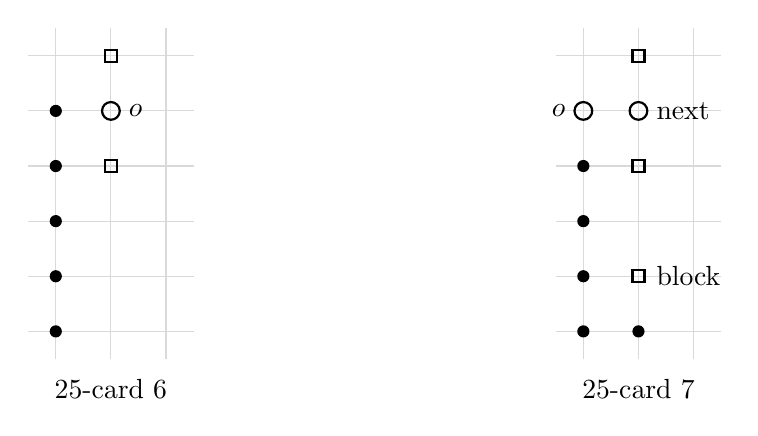
\begin{tikzpicture}[x=7mm,y=7mm]
 \begin{scope}
  \draw[gray!30,step=1] (-1.5,-4.5) grid (1.5,1.5);
  \foreach \y in {-4,-3,-2,-1,0}
    \fill (-1,\y) circle (2.2pt);
  \draw[thick] (0,0) circle (3.2pt);
  \node[right] at (0.15,0) {$o$};
  \foreach \y in {-1,1}
    \draw[thick] (-0.11,\y-0.11) rectangle (0.11,\y+0.11);
  \node[below] at (0,-4.7) {$25$-card $6$};
 \end{scope}
 \begin{scope}[xshift=6cm]
  \draw[gray!30,step=1] (-0.5,-4.5) grid (2.5,1.5);
  \foreach \y in {-4,-3,-2,-1}
    \fill (0,\y) circle (2.2pt);
  \fill (1,-4) circle (2.2pt);
  \draw[thick] (0,0) circle (3.2pt);
  \node[left] at (-0.15,0) {$o$};
  \draw[thick] (0.89,-3.11) rectangle (1.11,-2.89);
  \node[right] at (1.15,-3) {block};
  \draw[thick] (1,0) circle (3.2pt);
  \node[right] at (1.15,0) {next};
  \foreach \y in {-1,1}
    \draw[thick] (0.89,\y-0.11) rectangle (1.11,\y+0.11);
  \node[below] at (1,-4.7) {$25$-card $7$};
 \end{scope}
\end{tikzpicture}
\caption{The elementary reduced cards.  Solid disks are the required
Maker cells.  In card $6$, attacking the open disk $o$ gives the two
square-marked finishes.  In card $7$, the attack at $o$ threatens the
square $(1,-3)$; after that block, the open disk $(1,0)$ starts the
translated card $6$, with finishes at the other two squares.}
\label{r25:elementary-figure}
\end{figure}

\subsection{The complete finite reconstruction and its endpoint}
\label{r25:reconstruction}

We now apply the same recurrence to the entire literal, retaining
every row.  The supplied primary program
\path{verification/supporting/route25/verify_certificate.py} and independent
program \path{verification/supporting/route25/independent_certificate.py}
reconstruct its finite sets and heights.  Their checks include the
decimal grammar, every backward reference and anchor, the marker
numbers, the required number of rows, and the exact endpoint.
Malformed or truncated input is rejected; Appendix~\ref{app:checker}
gives the verification commands and their scope.  Their finite arithmetic
supports the set identities below; the reason these sets give a game
strategy is Proposition~\ref{r25:composition} and the induction just
proved, independently of either program.

The complete reconstruction has $2016$ cards and $5862$ placed child
terms.  The number of cards of each required-set size is
\begin{equation}\label{r25:histogram}
\begin{array}{c|rrrrrrrrrrr}
 |P_i|&0&1&2&3&4&5&6&7&8&9&10\\ \hline
 \text{number}&1&5&52&217&448&523&416&219&103&30&2.
\end{array}
\end{equation}
The last card can also be inspected through the much smaller
terminal table.  Its $28$ children comprise exactly the following
five groups in the printed order.  Each listed code has anchor index
$k=0$.  The last column gives the size of the intersection of all
placed reduced envelopes through the end of that row of the table.
\begin{table}[htbp]
\centering
\begin{tabular}{rcrrr}
\toprule
Child $j$&Codes $r$&$|E_j|$&$h_j$&Cumulative intersection\\
\midrule
$1874$&$0,1,2,5$&$292$&$24$&$184$\\
$1985$&$0,2,4,6$&$162$&$19$&$96$\\
$1996$&$0,1,2,5$&$117$&$15$&$49$\\
$1998$&$0,1,2,3,4,5,6,7$&$119$&$20$&$32$\\
$2014$&$0,1,2,3,4,5,6,7$&$76$&$14$&$0$\\
\bottomrule
\end{tabular}
\caption{All children of $25$-card $2015$.  The common reduced
envelope disappears after the last group.}
\label{r25:terminal-table}
\end{table}
The required sets of these five child cards are
\begin{equation}\label{r25:singleton-requirements}
 P_{1874}=P_{1985}=P_{1996}=\{(-1,0)\},\qquad
 P_{1998}=\{(0,1)\},\qquad P_{2014}=\{(1,0)\}.
\end{equation}
Every placed requirement is therefore $\{o\}$.  The table gives
$U=\{o\}$ and $I=\varnothing$, hence $H=\{o\}$ and
\begin{equation}\label{r25:terminal}
 P_{2015}=\varnothing,\qquad |E_{2015}|=389,\qquad h_{2015}=25.
\end{equation}
The last height is $1+24$, not a bound obtained by identifying this
certificate with either of the other two constructions.

For an explicit description of the final finite region, its section
at ordinate $y$ is empty when $|y|>11$; otherwise it is the set of
integer abscissae in the following table:
\begin{center}
\begin{tabular}{c|c@{\qquad}c|c}
\toprule
$|y|$&Abscissae $x$&$|y|$&Abscissae $x$\\
\midrule
$0$&$[-10,10]$&$6$&$[-9,9]$\\
$1$&$[-11,11]$&$7$&$[-7,7]$\\
$2$&$[-10,10]$&$8$&$[-6,6]$\\
$3$&$[-11,11]$&$9$&$[-6,6]$\\
$4$&$[-10,10]$&$10$&$[-5,5]$\\
$5$&$[-10,10]$&$11$&$\{-3,-1,1,3\}$\\
\bottomrule
\end{tabular}
\end{center}
Here intervals mean all integer points.  The row counts give
$21+2(23+21+23+21+21+19+15+13+13+11+4)=389$.

\begin{proposition}[The $25$-move strategy]\label{r25:bound}
There is one ordinary Maker policy on the infinite square board that,
from the empty position, completes a copy of $S$ within $25$ actual
fresh Maker claims against every legal Breaker continuation.  In the
fixed-endpoint formulation, after extending the policy by fresh moves
beyond an earlier win, the Maker set after its $25$th claim contains
a target whenever the first $24$ Breaker replies are legal along the
policy.
\end{proposition}

\begin{proof}
Induction using~\eqref{r25:bases} and
Proposition~\ref{r25:composition} proves the validity of all $2016$
cards.  Equation~\eqref{r25:terminal} therefore applies at the empty
position.  To fix one policy before the opponent's choices, fix an
enumeration of $\Z^2$ and the printed order of every child list.
Start with card $2015$ in its identity placement.  At a composite
card in placement $F$, take $F(o)$ if free, or the first free cell
of the enumeration if $F(o)$ is already owned.  Stop at a target.
If play continues, after the next legal Breaker reply choose the
first child $(j,r)$ whose placed reduced envelope avoids the current
Breaker set.  The composition proof guarantees its existence and its
required ownership.  Replace the active placement by
$F\circ\Phi_{j,r}$.  At a base, its hole is either already filled,
giving a target, or can be taken to finish one.

Each nonterminal descent consumes one actual fresh Maker claim,
including every replacement, and decreases the height.  No path from
height $25$ needs more than $25$ such claims.  As in
Section~\ref{sec:strategy}, the active card and placement are determined
by replaying the complete history.  On a history inconsistent with
the policy, or beyond a completed target, prescribe the first free
cell instead.  This makes the policy globally legal on finite legal
histories and fixes it independently of future replies.

If the first win is on claim $m\leq25$, exactly $m-1$ replies have
preceded it.  Thus only $24$ replies can be needed.  Under the extended
policy an earlier target persists, proving the fixed-endpoint
statement without any assumption on a $25$th Breaker reply.
\end{proof}

\subsection{Why only five first-reply classes need extra cards}
\label{r25:opening}

The final row can be understood geometrically as a cover of all first
Breaker replies.  After Maker takes $o$, each of the eight placements
$\Phi_{2014,d}$, $0\leq d<8$, has required set $\{o\}$.
Let $D$ be the intersection of their reduced envelopes.  The exact
finite calculation is
\begin{equation}\label{r25:opening-common}
 \begin{split}
 D={}&\{(\pm t,0),(0,\pm t):t=1,2,3\}\\
    &\ \cup\{(\pm1,\pm1)\}
      \cup\{(\pm2,\pm1),(\pm1,\pm2)\},
 \end{split}
\end{equation}
with independent signs.  It contains $24$ cells.  In particular
the sorted absolute coordinates, larger first, have exactly the five
values
\[
 (1,0),\quad(1,1),\quad(2,0),\quad(2,1),\quad(3,0).
\]
The set $D$ is invariant under all signed permutations: composing any
one of those permutations with the eight placements merely permutes
them.  Equation~\eqref{r25:opening-common} is a finite set identity,
so it covers unbounded first replies as well: for every $b\notin D$,
at least one of the eight envelopes omits $b$.  That placement of
card $2014$ is already available, giving at most $14$ further claims.

For the five remaining classes, the following placements omit the
listed first Breaker cell.  All use $k=0$ and have placed required
set $\{o\}$.
\begin{table}[htbp]
\centering
\begin{tabular}{cccrr}
\toprule
First Breaker cell&Child $j$&$d$&Next attack&Further bound $h_j$\\
\midrule
$(1,0)$&$1874$&$2$&$(-1,0)$&$24$\\
$(1,1)$&$1985$&$6$&$(-1,0)$&$19$\\
$(2,0)$&$1996$&$2$&$(-1,0)$&$15$\\
$(2,1)$&$1998$&$2$&$(0,-1)$&$20$\\
$(3,0)$&$1996$&$2$&$(-1,0)$&$15$\\
\bottomrule
\end{tabular}
\caption{The five exceptional opening classes for the $25$-move
construction.  Each bound begins at Maker's second turn.}
\label{r25:opening-table}
\end{table}
For example, the first placement is
$\Phi_{1874,2}(x,y)=(-x-1,y)$ because its anchor is $(-1,0)$;
the fourth is $\Phi_{1998,2}(x,y)=(-x,y-1)$ because its anchor is
$(0,1)$.  These formulas give the displayed attacks directly.
For an arbitrary reply in one of the five classes, choose a signed
permutation $Q$ taking its representative to that reply and use the
placement $Q\circ\Phi_{j,d}$.  It still requires only $o$, and its
envelope omits that reply.  Thus the table and the eight placements
of card $2014$ give a direct whole-board opening proof, with largest
total $1+24=25$.  The terminal row in
Table~\ref{r25:terminal-table} encodes a finite opening cover of this
kind using its specified $28$ placements.

\subsection{Two continuations that leave the initial line}
\label{r25:nonlocal}

We finish by following two actual children of card $1874$.  This
makes the composition of coordinate maps visible and shows why an
implementation must retain the complete envelopes.  Suppose Maker
has played $o$, Breaker has replied $(1,0)$, and Maker uses the first
row of Table~\ref{r25:opening-table} to attack $(-1,0)$.  The current
outer placement is
\[
 F(x,y)=\Phi_{1874,2}(x,y)=(-x-1,y),
 \qquad M=\{o,(-1,0)\},\qquad B=\{(1,0)\}
\]
before Breaker's next reply.  The two following continuations are
present in the literal row for card $1874$:
\begin{center}
\begin{tabular}{ccccc}
\toprule
Next reply&Child $j$&Code $r$&Anchor $a_{j,k}$&Next attack\\
\midrule
$(-1,-1)$&$1716$&$8$&$(-2,-1)$&$(-3,1)$\\
$(-2,0)$&$1752$&$3$&$(-2,0)$&$(-1,2)$\\
\bottomrule
\end{tabular}
\end{center}

For the first, the native required set is
$P_{1716}=\{(-3,-1),(-2,-1)\}$.  Since $8=8\cdot1+0$, the
lexicographic anchor is the second point, $(-2,-1)$, and
\[
 \Phi_{1716,8}(x,y)=(x+2,y+1),\qquad
 (F\circ\Phi_{1716,8})(x,y)=(-x-3,y+1).
\]
The transformed requirement is precisely $\{o,(-1,0)\}$.
The reduced envelope has $256$ cells and satisfies the exact check
\begin{equation}\label{r25:avoidance1}
 (F\circ\Phi_{1716,8})(E_{1716})
       \cap\{(1,0),(-1,-1)\}=\varnothing.
\end{equation}
Thus the old reply as well as the new reply is excluded, and the
transformed pivot is $(-3,1)$.  It is distinct from all four cells
then owned by either player.  Card $1716$ supplies a height-$23$
continuation after the first two Maker claims, consistent with the
total bound $25$.

For the second, $P_{1752}=\{(-2,0),(-2,1)\}$ and $r=3$ selects
the first anchor and the swap-first map $R_3(x,y)=(-y,x)$.  Hence
\[
 \Phi_{1752,3}(x,y)=(-y,x+2),\qquad
 (F\circ\Phi_{1752,3})(x,y)=(y-1,x+2).
\]
Its requirement is again exactly $\{o,(-1,0)\}$, while its
$93$-cell reduced envelope satisfies
\begin{equation}\label{r25:avoidance2}
 (F\circ\Phi_{1752,3})(E_{1752})
       \cap\{(1,0),(-2,0)\}=\varnothing.
\end{equation}
Its pivot $(-1,2)$ is free, and this child has height $15$.
Equations~\eqref{r25:avoidance1}--\eqref{r25:avoidance2} use the
complete reconstructed envelopes, not just the new pivot or the
required pair of Maker cells.

The two replies here are legal examples, not forced Breaker choices.
For either example the indicated child is usable; the globally fixed
first-surviving-child policy may select an earlier usable child in
the same row.  Other replies are covered by the full child list and
Proposition~\ref{r25:composition}.  Neither the game nor this
certificate restricts Maker's holdings to a connected shape: these
two attacks deliberately leave the initial horizontal pair.
